% AUTO-GENERATED by figs/make_figures.py from sim/results/*.csv
% and sim/tier2/results/*.csv. Re-run the generator to refresh.
% Colour palette: Okabe-Ito (colour-blind safe, prints legibly in grey).
\definecolor{cA}{RGB}{0,114,178}
\definecolor{cB}{RGB}{213,94,0}
\definecolor{cC}{RGB}{0,158,115}
\definecolor{cD}{RGB}{204,121,167}
\definecolor{cE}{RGB}{230,159,0}
\pgfplotsset{
  paperfig/.style={
    grid=both, grid style={black!10},
    legend cell align=left,
    legend style={font=\scriptsize, fill=white, fill opacity=0.92,
                  text opacity=1, draw=black!45, inner xsep=3pt,
                  inner ysep=1.6pt, rounded corners=1pt},
    tick label style={font=\footnotesize},
    label style={font=\footnotesize},
  }
}

\begin{figure}[t]\centering
\begin{tikzpicture}
\begin{axis}[paperfig,width=\columnwidth,height=0.66\columnwidth,
  xlabel={duty cycle $\delta$},ylabel={age (normalized, $P{=}1$)},
  legend style={at={(0.5,-0.26)},anchor=north,legend columns=2},
  error bars/y dir=both,error bars/y explicit]
\addplot[cA,only marks,mark=*,mark size=1.5pt] coordinates {(0.02,0.9870100715269062) +- (0,3.1292142984718735e-05) (0.05,0.9569975439410504) +- (0,2.8138476284065702e-05) (0.075,0.9320010411719328) +- (0,2.902494335842732e-05) (0.1,0.9069955973162998) +- (0,1.893193054617168e-05) (0.2,0.8069971556041535) +- (0,2.4082530275375084e-05) (0.35,0.657020357263457) +- (0,2.364619973598577e-05) (0.5,0.5069971053296146) +- (0,2.473059005205108e-05)};
\addlegendentry{OPAoI (sim)}
\addplot[cA,no marks,thick,dashed] coordinates {(0.02,0.985) (0.05,0.955) (0.075,0.93) (0.1,0.905) (0.2,0.805) (0.35,0.655) (0.5,0.505)};
\addlegendentry{OPAoI $=T_s+P(1-\delta)$}
\addplot[cB,only marks,mark=square*,mark size=1.5pt] coordinates {(0.02,0.48721054412512643) +- (0,3.05966842493133e-05) (0.05,0.45824685360113504) +- (0,2.693793306118609e-05) (0.075,0.4348135198357405) +- (0,2.655059400816846e-05) (0.1,0.4119961987610867) +- (0,1.6638518202369598e-05) (0.2,0.3269977862109709) +- (0,1.944432796664332e-05) (0.35,0.21826373712641028) +- (0,1.6032026469115834e-05) (0.5,0.13199933546467407) +- (0,1.2466013684464939e-05)};
\addlegendentry{mean AoI (sim)}
\addplot[cB,no marks,thick,densely dotted] coordinates {(0.02,0.48519999999999996) (0.05,0.45625) (0.075,0.43281250000000004) (0.1,0.41000000000000003) (0.2,0.32500000000000007) (0.35,0.21625000000000003) (0.5,0.13)};
\addlegendentry{mean AoI $=T_s+\tfrac{P}{2}(1-\delta)^2$}
\end{axis}
\end{tikzpicture}
\caption{Result~1 (E1/E2): simulated mean AoI and OPAoI vs.\ duty cycle
match the closed forms; the peak grows linearly and the mean
quadratically in $(1-\delta)$ (provisioning divergence). Markers are
Monte-Carlo means with 95\% CIs (smaller than markers).}
\label{fig:r1}
\end{figure}


\begin{figure}[t]\centering
\begin{tikzpicture}
\begin{axis}[paperfig,width=\columnwidth,height=0.6\columnwidth,
  xlabel={duty cycle $\delta$},ylabel={$\mathbb{E}[R_{\min}]/\mathbb{E}[R]$},
  legend pos=north east,grid=both,legend cell align=left]
\addplot[cA,only marks,mark=*,mark size=1.6pt] coordinates {(0.02,0.653362323347421) (0.05,0.6333883269504517) (0.1,0.6001979804547108) (0.2,0.5336253055696409) (0.35,0.433159970801058) (0.5,0.33323957490210027)};
\addlegendentry{sim}
\addplot[cB,no marks,thick,dashed] coordinates {(0.02,0.6533333333333333) (0.05,0.6333333333333333) (0.1,0.6) (0.2,0.5333333333333333) (0.35,0.43333333333333335) (0.5,0.3333333333333333)};
\addlegendentry{$\tfrac{2}{3}(1-\delta)$}
\end{axis}
\end{tikzpicture}
\caption{Result~2 (E4): the two-copy gain. Simulated
$\mathbb{E}[R_{\min}]/\mathbb{E}[R]$ matches the two-copy
ratio $\tfrac{2}{3}(1-\delta)$; replication saves most at sparse
contacts ($\delta\to0$).}
\label{fig:r2gain}
\end{figure}


\begin{figure}[t]\centering
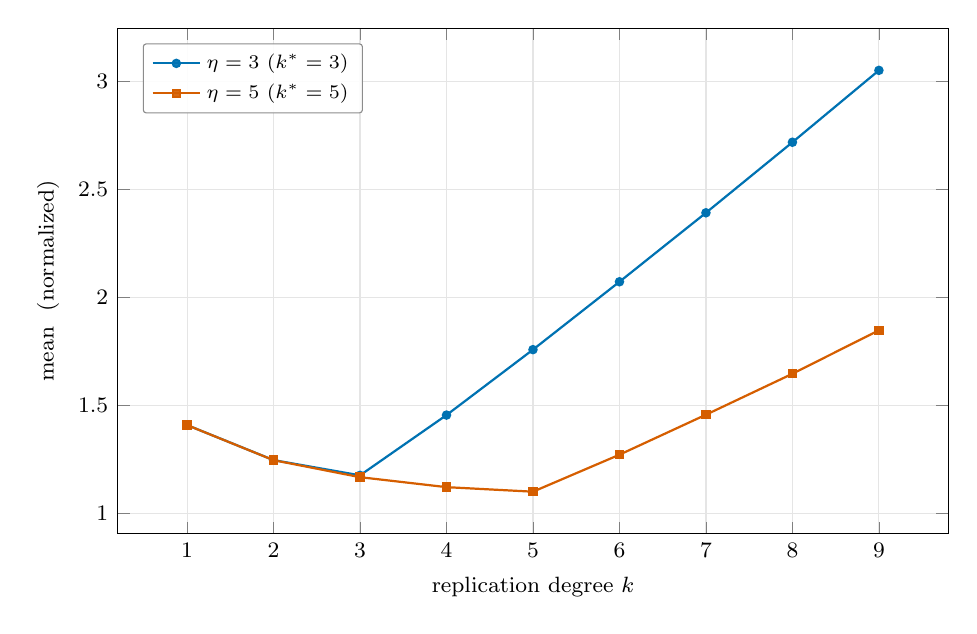
\begin{tikzpicture}
\begin{axis}[paperfig,width=\columnwidth,height=0.66\columnwidth,
  xlabel={replication degree $k$},ylabel={mean $\PAoIper$ (normalized)},
  legend pos=north west,grid=both,legend cell align=left,xtick=data]
\addplot[thick,cA,mark=*,mark size=1.3pt] coordinates {(1.0,1.410314663389778) (2.0,1.248192570863487) (3.0,1.1777586195908003) (4.0,1.4564704134531814) (5.0,1.7592147238268279) (6.0,2.073176697683509) (7.0,2.3922001335971532) (8.0,2.7185592470423137) (9.0,3.0510884750494167)};
\addlegendentry{$\eta=3$ ($k^\ast=3$)}
\addplot[thick,cB,mark=square*,mark size=1.3pt] coordinates {(1.0,1.4101859347850572) (2.0,1.2478719880669222) (3.0,1.1692371885105677) (4.0,1.123112635056019) (5.0,1.1020916179657483) (6.0,1.2732102430111434) (7.0,1.458191515479616) (8.0,1.6476294592829408) (9.0,1.8487261126269243)};
\addlegendentry{$\eta=5$ ($k^\ast=5$)}
\end{axis}
\end{tikzpicture}
\caption{Result~3 (E7): the integrated energy+replication+AoI objective
is unimodal in $k$ with minimum at one of the two integers bracketing
$\eta$; pushing
$k$ past the energy budget starves future contacts and raises the peak.}
\label{fig:r3unimodal}
\end{figure}


\begin{figure}[t]\centering
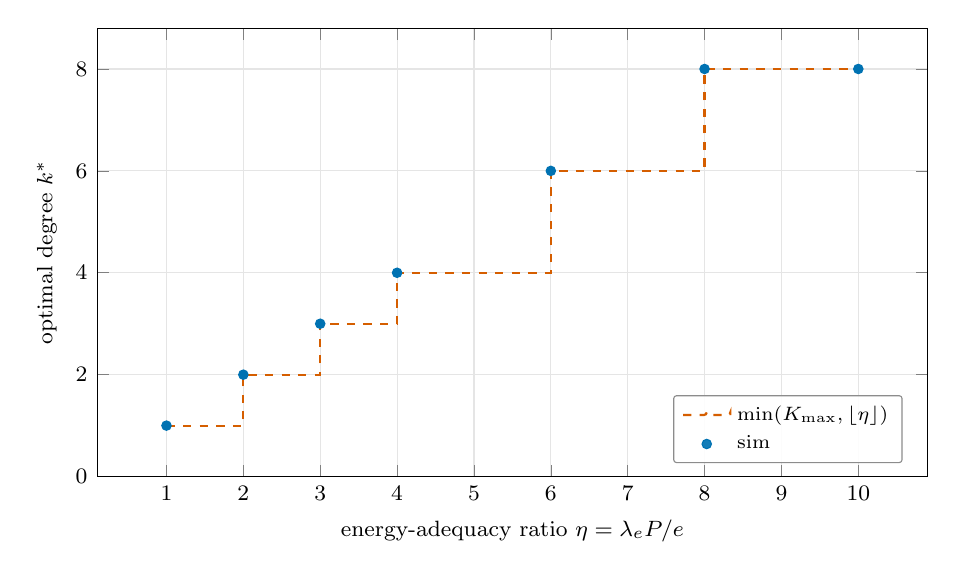
\begin{tikzpicture}
\begin{axis}[paperfig,width=\columnwidth,height=0.6\columnwidth,
  xlabel={energy-adequacy ratio $\eta=\lambda_e P/e$},ylabel={optimal degree $k^\ast$},
  legend pos=south east,grid=both,legend cell align=left,ymin=0]
\addplot[cB,no marks,thick,dashed,const plot] coordinates {(1.0,1.0) (2.0,2.0) (3.0,3.0) (4.0,4.0) (6.0,6.0) (8.0,8.0) (10.0,8.0)};
\addlegendentry{$\min(K_{\max},\lfloor\eta\rfloor)$}
\addplot[cA,only marks,mark=*,mark size=1.7pt] coordinates {(1.0,1.0) (2.0,2.0) (3.0,3.0) (4.0,4.0) (6.0,6.0) (8.0,8.0) (10.0,8.0)};
\addlegendentry{sim}
\end{axis}
\end{tikzpicture}
\caption{Result~3 (E8): $k^\ast(\eta)$ is non-decreasing in the
harvest-to-contact ratio and saturates at $K_{\max}{=}8$ once energy
ceases to bind.}
\label{fig:r3kstar}
\end{figure}


\begin{figure}[t]\centering
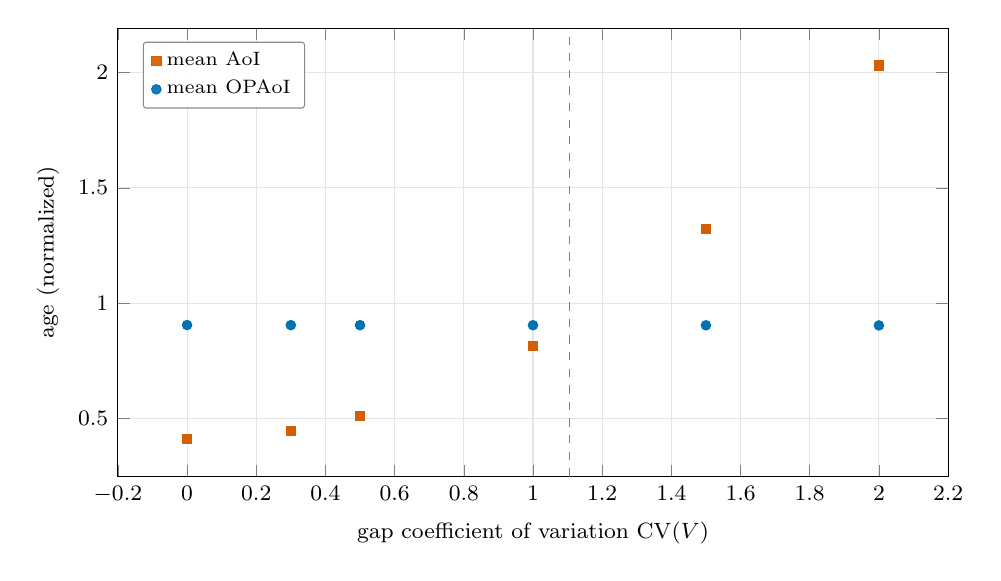
\begin{tikzpicture}
\begin{axis}[paperfig,width=\columnwidth,height=0.6\columnwidth,
  xlabel={gap coefficient of variation $\mathrm{CV}(V)$},
  ylabel={age (normalized)},legend pos=north west,grid=both,
  legend cell align=left]
\addplot[cB,only marks,mark=square*,mark size=1.7pt] coordinates {(0.0,0.41) (0.3,0.44625348238863416) (0.5,0.5108772600771613) (1.0,0.8149996897795648) (1.5,1.3224004704089134) (2.0,2.030147837685105)};
\addlegendentry{mean AoI}
\addplot[cA,only marks,mark=*,mark size=1.7pt] coordinates {(0.0,0.9049999999999999) (0.3,0.9046423617422175) (0.5,0.9044223082534586) (1.0,0.9043348492407165) (1.5,0.9039569330472569) (2.0,0.9033825094312596)};
\addlegendentry{mean OPAoI}
\draw[gray,dashed] (axis cs:1.106,\pgfkeysvalueof{/pgfplots/ymin}) -- (axis cs:1.106,\pgfkeysvalueof{/pgfplots/ymax});
\end{axis}
\end{tikzpicture}
\caption{The AoI/OPAoI inversion (E12). Mean OPAoI ($=T_s+
\mathbb{E}[V]$) is flat in the gap variability, while mean AoI grows
with it; they cross at the exact threshold
$\mathrm{CV}^2(V)=1+2\mathbb{E}[U]/\mathbb{E}[V]$ (dashed:
$\mathrm{CV}\approx1.11$ for the plotted $\mathbb{E}[U]/\mathbb{E}[V]=1/9$),
so for high-variance
terrestrial contacts the outage peak sits {\itshape below}
average AoI.}
\label{fig:inversion}
\end{figure}


\begin{figure}[t]\centering
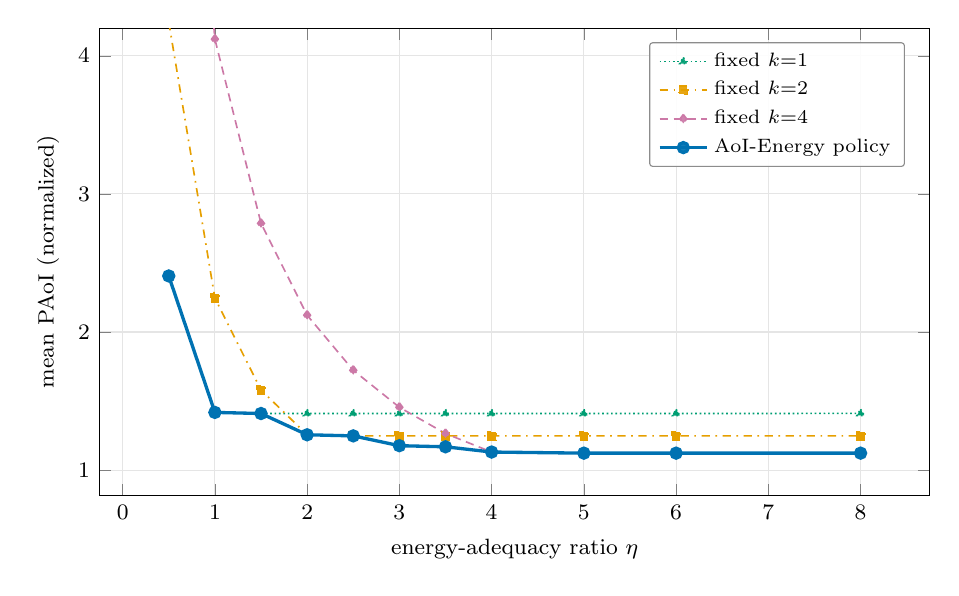
\begin{tikzpicture}
\begin{axis}[paperfig,width=\columnwidth,height=0.62\columnwidth,
  xlabel={energy-adequacy ratio $\eta$},ylabel={mean PAoI (normalized)},
  legend pos=north east,grid=both,legend cell align=left,ymax=4.2]
\addplot[cC,semithick,densely dotted,mark=triangle*,mark size=1.5pt] coordinates {(0.5,2.406) (1.0,1.418) (1.5,1.410) (2.0,1.410) (2.5,1.410) (3.0,1.410) (3.5,1.410) (4.0,1.410) (5.0,1.410) (6.0,1.410) (8.0,1.411)};
\addlegendentry{fixed $k{=}1$}
\addplot[cE,semithick,dashdotted,mark=square*,mark size=1.5pt] coordinates {(0.5,4.244) (1.0,2.246) (1.5,1.580) (2.0,1.256) (2.5,1.248) (3.0,1.248) (3.5,1.248) (4.0,1.248) (5.0,1.248) (6.0,1.248) (8.0,1.248)};
\addlegendentry{fixed $k{=}2$}
\addplot[cD,semithick,densely dashed,mark=diamond*,mark size=1.6pt] coordinates {(0.5,8.111) (1.0,4.121) (1.5,2.787) (2.0,2.122) (2.5,1.723) (3.0,1.455) (3.5,1.265) (4.0,1.131) (5.0,1.123) (6.0,1.123) (8.0,1.123)};
\addlegendentry{fixed $k{=}4$}
\addplot[cA,very thick,mark=*,mark size=1.8pt] coordinates {(0.5,2.406) (1.0,1.418) (1.5,1.410) (2.0,1.256) (2.5,1.248) (3.0,1.177) (3.5,1.169) (4.0,1.131) (5.0,1.123) (6.0,1.123) (8.0,1.123)};
\addlegendentry{AoI-Energy policy}
\end{axis}
\end{tikzpicture}
\caption{The AoI-Energy policy selects the replication degree from the
closed-form rule $k_{\mathrm{pol}}(\eta)=\arg\min_k\mathcal{A}(k)$
(no search); it matched the per-$\eta$ exhaustive optimum in all 11 cases
and is the lower envelope of every fixed-degree curve. A single fixed $k$
is wasteful when energy is scarce (large $k$ starves) or stale when it is
abundant (small $k$ misses the order-statistic gain); the adaptive policy
is best at every energy level.}
\label{fig:policy}
\end{figure}


\begin{figure}[t]\centering
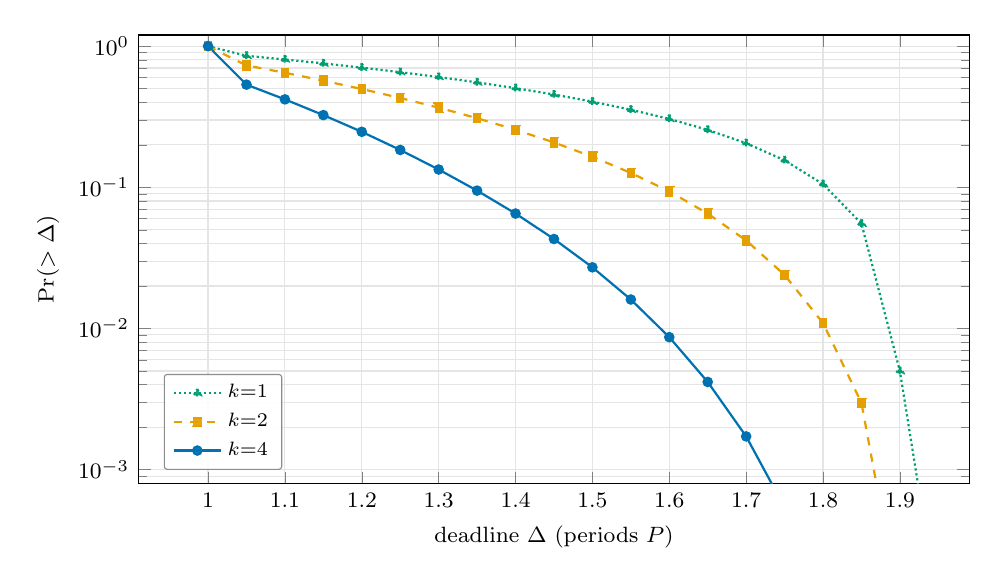
\begin{tikzpicture}
\begin{semilogyaxis}[paperfig,width=\columnwidth,height=0.6\columnwidth,
  xlabel={deadline $\Delta$ (periods $P$)},
  ylabel={$\Pr(\PAoIper>\Delta)$},legend pos=south west,grid=both,
  legend cell align=left,ymin=0.0008,ymax=1.2]
\addplot[cC,thick,densely dotted,mark=triangle*,mark size=1.5pt] coordinates {(1.0,1.00000) (1.05,0.85442) (1.1,0.80444) (1.15,0.75449) (1.2,0.70461) (1.25,0.65425) (1.3,0.60426) (1.35,0.55411) (1.4,0.50408) (1.45,0.45433) (1.5,0.40460) (1.55,0.35457) (1.6,0.30521) (1.65,0.25518) (1.7,0.20550) (1.75,0.15537) (1.8,0.10531) (1.85,0.05534) (1.9,0.00499) (1.95,0.00010) (2.0,0.00010)};
\addlegendentry{$k{=}1$}
\addplot[cE,thick,dashed,mark=square*,mark size=1.5pt] coordinates {(1.0,1.00000) (1.05,0.73057) (1.1,0.64790) (1.15,0.56975) (1.2,0.49702) (1.25,0.42933) (1.3,0.36668) (1.35,0.30882) (1.4,0.25571) (1.45,0.20794) (1.5,0.16468) (1.55,0.12647) (1.6,0.09356) (1.65,0.06516) (1.7,0.04208) (1.75,0.02393) (1.8,0.01093) (1.85,0.00297) (1.9,0.00010) (1.95,0.00010) (2.0,0.00010)};
\addlegendentry{$k{=}2$}
\addplot[cA,thick,mark=*,mark size=1.5pt] coordinates {(1.0,1.00000) (1.05,0.53382) (1.1,0.41980) (1.15,0.32479) (1.2,0.24730) (1.25,0.18397) (1.3,0.13372) (1.35,0.09478) (1.4,0.06520) (1.45,0.04305) (1.5,0.02712) (1.55,0.01604) (1.6,0.00868) (1.65,0.00418) (1.7,0.00172) (1.75,0.00054) (1.8,0.00011) (1.85,0.00010) (1.9,0.00010) (1.95,0.00010) (2.0,0.00010)};
\addlegendentry{$k{=}4$}
\end{semilogyaxis}
\end{tikzpicture}
\caption{PAoI tail (deadline-violation probability) at energy-abundant
$\eta$: replication pulls in the tail via the order statistic. The
probability of exceeding a $1.5P$ freshness deadline falls from $0.40$
($k{=}1$) to $0.16$ ($k{=}2$) to $0.027$ ($k{=}4$)---a $15\times$
reduction---and the $99$th-percentile PAoI drops from $1.90P$ to $1.59P$.
Mean PAoI alone understates the benefit of replication for
mission-critical traffic.}
\label{fig:ccdf}
\end{figure}


\begin{figure}[t]\centering
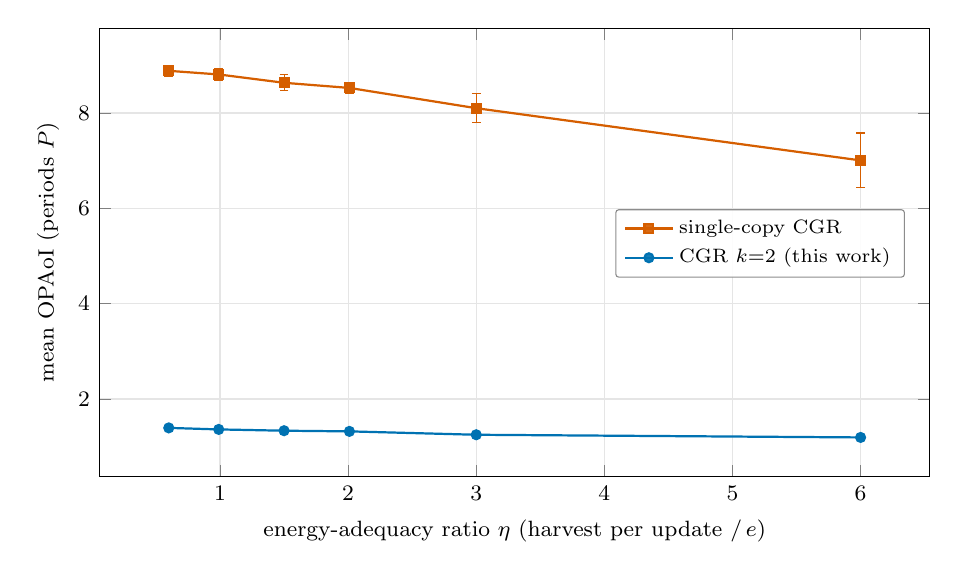
\begin{tikzpicture}
\begin{axis}[paperfig,width=\columnwidth,height=0.6\columnwidth,
  xlabel={energy-adequacy ratio $\eta$ (harvest per update $/\,e$)},
  ylabel={mean OPAoI (periods $P$)},
  legend style={at={(0.97,0.52)},anchor=east},
  error bars/y dir=both,error bars/y explicit]
\addplot[cB,thick,mark=square*,mark size=1.6pt] coordinates {(0.6,8.886) +- (0,0.110) (0.99,8.810) +- (0,0.116) (1.5,8.635) +- (0,0.166) (2.01,8.527) +- (0,0.108) (3.0,8.102) +- (0,0.303) (6.0,7.006) +- (0,0.575)};
\addlegendentry{single-copy CGR}
\addplot[cA,thick,mark=*,mark size=1.6pt] coordinates {(0.6,1.393) +- (0,0.034) (0.99,1.361) +- (0,0.022) (1.5,1.334) +- (0,0.038) (2.01,1.320) +- (0,0.030) (3.0,1.249) +- (0,0.020) (6.0,1.193) +- (0,0.037)};
\addlegendentry{CGR $k{=}2$ (this work)}
\end{axis}
\end{tikzpicture}
\caption{Replication benefit in a real CGR stack with our CGR-native
$k$-copy router (dtnsim, random relay faults, source energy gate; 10
seeds, 95\% CIs). Sending two copies over the two best distinct CGR
routes cuts mean OPAoI by roughly $6\times$ versus single-copy across the
whole energy range---the order statistic hedges relay faults. Because the
per-transmission energy gate defers the second copy when the battery is
low (rather than dropping the update), the benefit degrades gracefully as
$\eta$ falls instead of inverting. This experiment isolates the
fault-hedging \emph{mechanism}; it is not a test of the atomic
all-or-nothing policy of \eqref{eq:kstar}, whose over-replication
penalty appears in Fig.~\ref{fig:r3atomic}.}
\label{fig:r3tier2}
\end{figure}


\begin{figure}[t]\centering
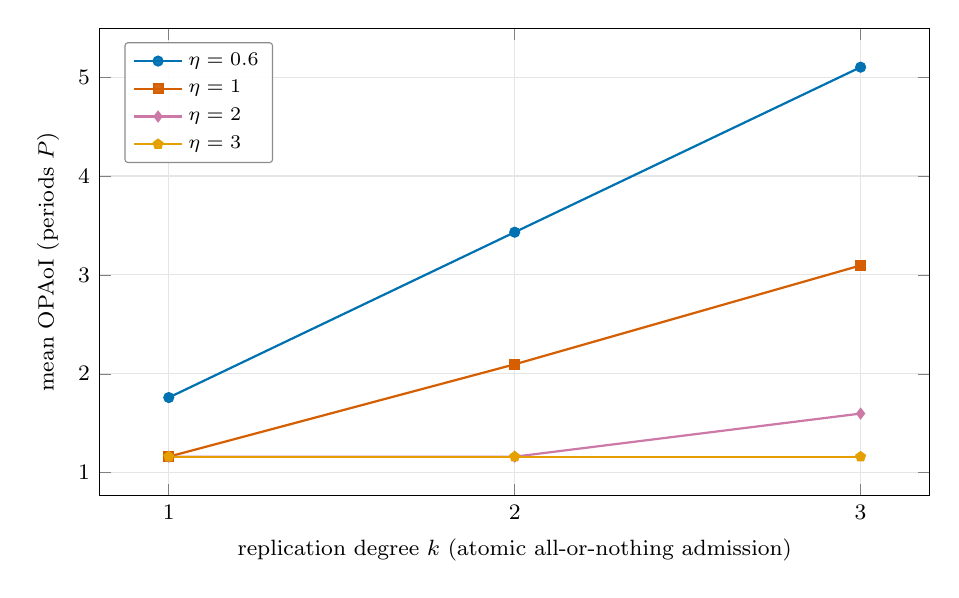
\begin{tikzpicture}
\begin{axis}[paperfig,width=\columnwidth,height=0.62\columnwidth,
  xlabel={replication degree $k$ (atomic all-or-nothing admission)},
  ylabel={mean OPAoI (periods $P$)},legend pos=north west,grid=both,
  legend cell align=left,xtick={1,2,3}]
\addplot[thick,cA,mark=*,mark size=1.6pt] coordinates {(1,1.760) (2,3.432) (3,5.101)};
\addlegendentry{$\eta=0.6$}
\addplot[thick,cB,mark=square*,mark size=1.6pt] coordinates {(1,1.162) (2,2.096) (3,3.096)};
\addlegendentry{$\eta=1$}
\addplot[thick,cD,mark=diamond*,mark size=1.6pt] coordinates {(1,1.162) (2,1.162) (3,1.598)};
\addlegendentry{$\eta=2$}
\addplot[thick,cE,mark=pentagon*,mark size=1.6pt] coordinates {(1,1.162) (2,1.162) (3,1.162)};
\addlegendentry{$\eta=3$}
\end{axis}
\end{tikzpicture}
\caption{Tier-2 atomic threshold test (real CGR, fault-free
3-relay staggered diamond, update-atomic admission: launch $k$ copies
iff the battery holds $k$ units, else skip the whole update; 5 seeds).
The over-replication penalty is now visible in the DTN stack:
at $\eta{=}1$, $k{=}3$ admits $35\%$ of updates (theory
$\min(1,\eta G_{\mathrm{gen}}/kP)$, matched to $<0.5\%$) and its
peak age is $2.7\times$ single-copy's. At $\eta\ge3$ the degrees tie
exactly: with a fault-free deterministic plan, oracle CGR's single copy
already rides the earliest route, so extra copies deliver stale
duplicates---the strict replication benefit requires route-outcome
uncertainty (Fig.~\ref{fig:r3tier2}).}
\label{fig:r3atomic}
\end{figure}


\begin{figure}[t]\centering
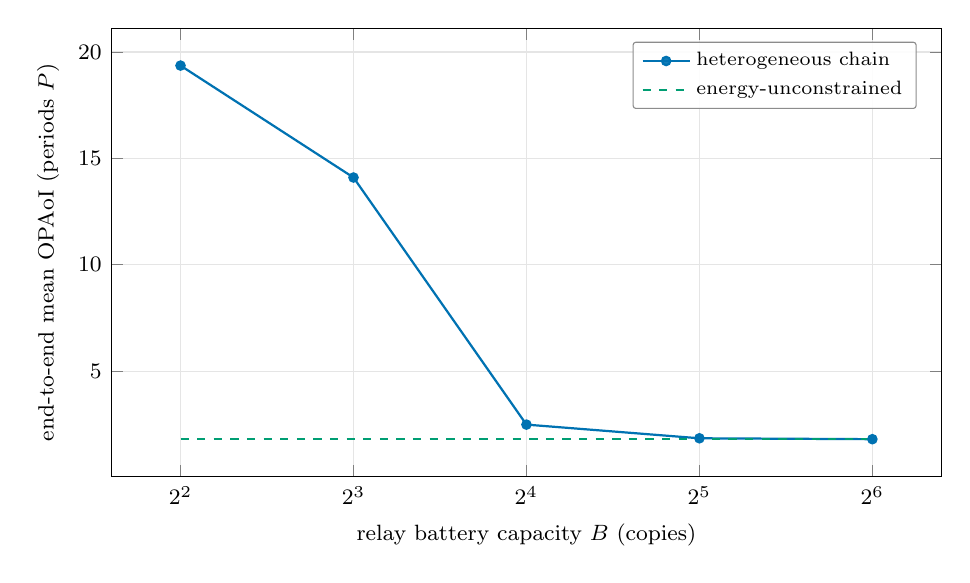
\begin{tikzpicture}
\begin{axis}[paperfig,width=\columnwidth,height=0.6\columnwidth,
  xlabel={relay battery capacity $B$ (copies)},
  ylabel={end-to-end mean OPAoI (periods $P$)},grid=both,
  xmode=log,log basis x=2,legend pos=north east,legend cell align=left]
\addplot[cA,thick,mark=*,mark size=1.5pt] coordinates {(4.0,19.361) (8.0,14.100) (16.0,2.487) (32.0,1.844) (64.0,1.802)};
\addlegendentry{heterogeneous chain}
\addplot[cC,thick,dashed,no marks] coordinates {(4,1.802) (64,1.802)};
\addlegendentry{energy-unconstrained}
\end{axis}
\end{tikzpicture}
\caption{Energy coupling in the full heterogeneous chain (sensor $\to$ UAV
mule $\to$ LEO $\to$ gateway in real CGR). A finite battery at the UAV/LEO
relays must cover the per-contact forwarding burst; below that, end-to-end
mean OPAoI degrades by $\sim\!11\times$ (and delivery collapses from $96\%$
to $31\%$). With sufficient battery it matches the energy-unconstrained
chain, whose mean delay confirms the additive composition
$\E[Y]{=}\E[R_1]{+}\E[R_2]{+}\E[R_3]$ to $1.1\%$.}
\label{fig:hetero}
\end{figure}
